\subsection{Design}
\label{sec:design}

%\sysname\ performs file-level deduplication for a Docker registry.
%
\begin{figure*}[t]
	\centering
		%\begin{minipage}{0.225\textwidth}
			\centering
			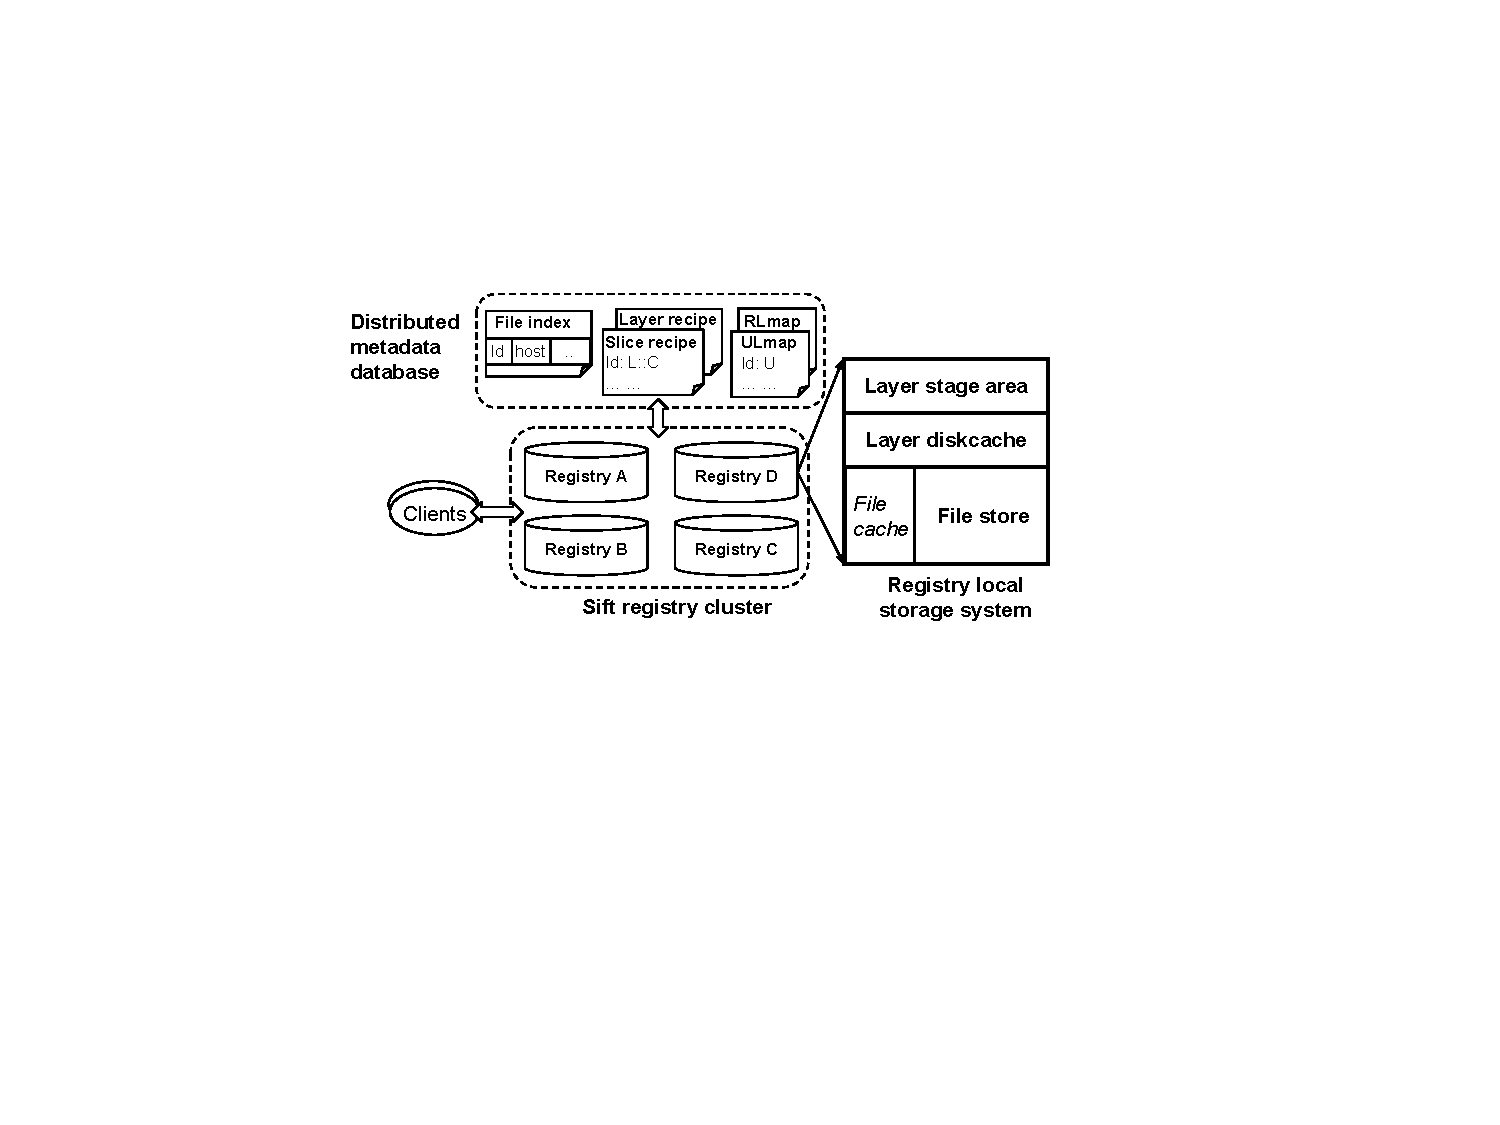
\includegraphics[width=0.9\textwidth]{graphs/sys-architecture.pdf}
%\vspace{-4pt}
			\caption{Architecture of \sysname.}
			%\label{fig:ref_count}
		%\end{minipage}
%	\begin{minipage}{0.225\textwidth}
%		\centering
%		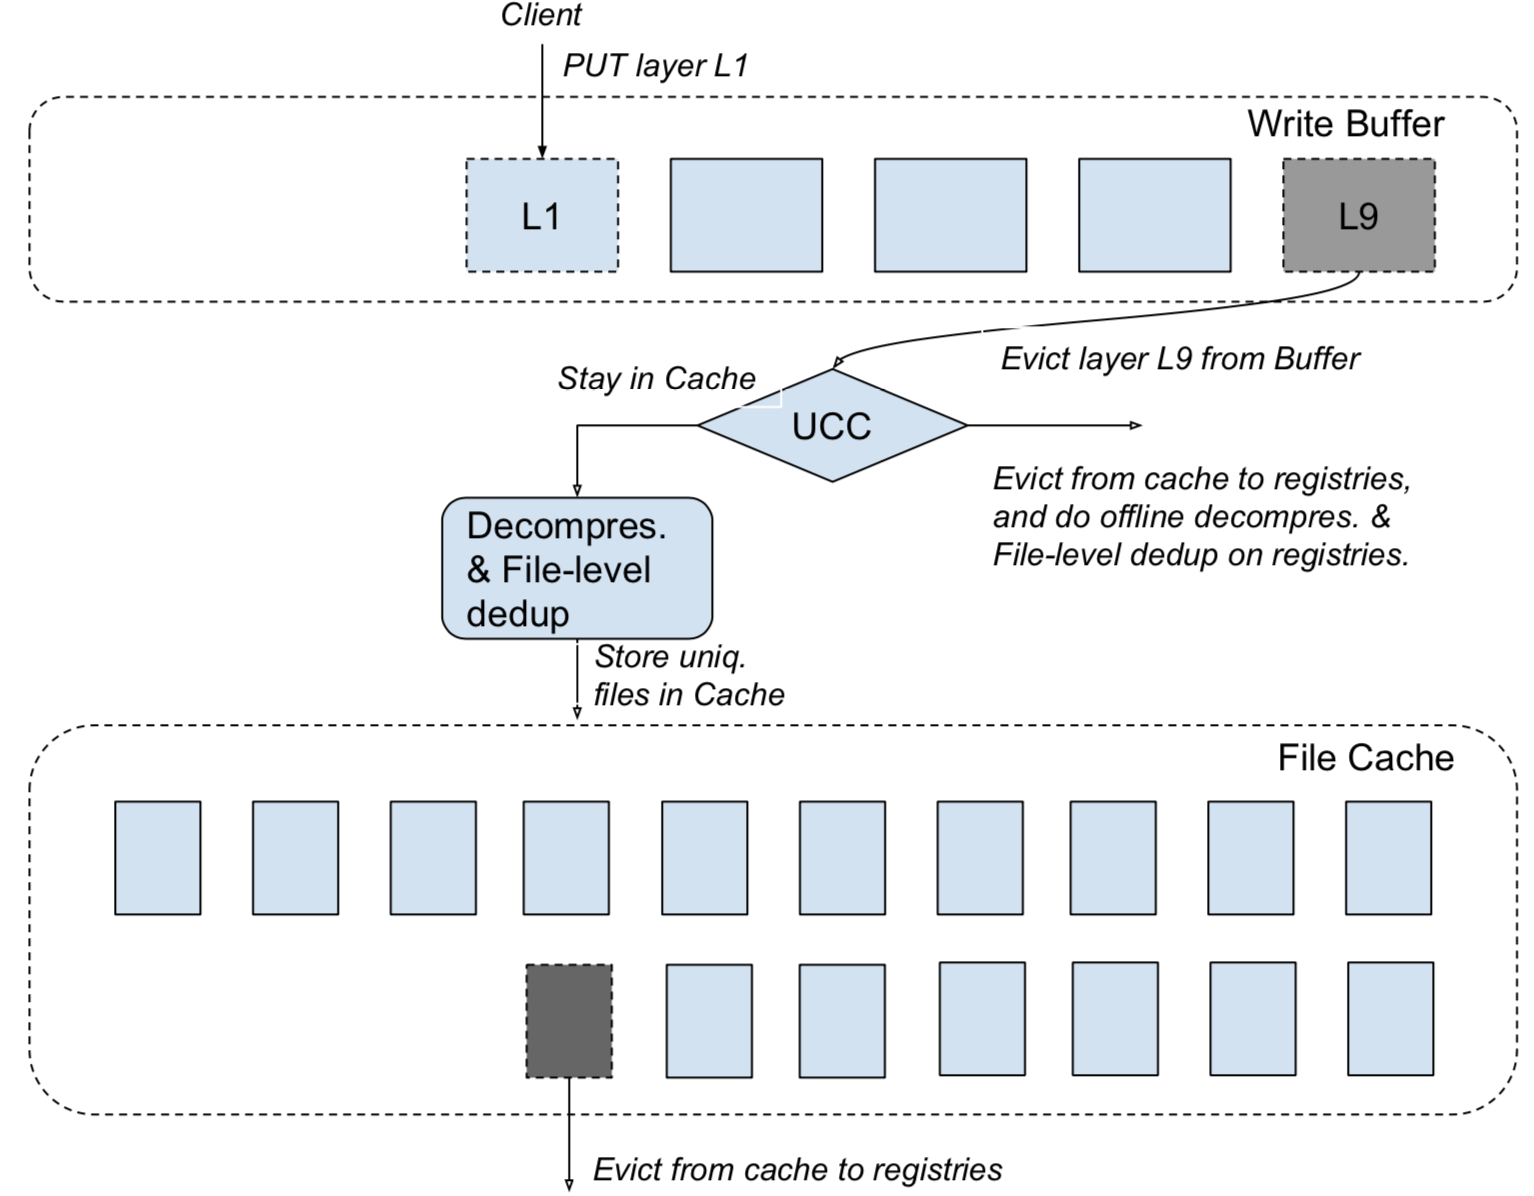
\includegraphics[width=1\textwidth]{graphs/slimmer-cache.png}
%		\caption{CDF of compress. and uncompress. layer size.}
%		\vspace{-3pt}
		\label{fig:sys-overview}
%\vspace{-4pt}
%	\end{minipage}
\end{figure*}

%We designed \sysname\ so that the interface between the Docker clients and the
%registry remains unchanged.
%
%As such, no modifications to the Docker clients are needed.
%
%Below we describe how \sysname\ handles layer pushes and
%pulls at the registry side.
%
%For the sake of this paper, we explain only the main steps omitting smaller
%details.

\paragraph{Push}
%
\sysname\ handles push requests asynchronously.
%
After receiving a layer from a client, it does not immediately unpack the layer.
%
Instead, it reliably stores the layer's compressed tarball in a persistent
\emph{staging area}.
%
A separate \emph{off-line} deduplication process iterates over the layers in
the staging area and performs the following steps for every layer:
%
\begin{compactenumerate}
  \item decompress and unpack the layer's tarball into individual files;
  \item compute a \emph{fingerprint} for every file in the layer;
  \item check all file fingerprints against the \emph{file index} to
	identify if identical files are already stored in \sysname;
  \item store non-deduplicated files in \sysname's storage;
  \item create and store a \emph{layer recipe} that includes the path,
	metadata, and fingerprint of every file in the layer;
  \item remove the layer's tarball from the staging area.
\end{compactenumerate}

%The advantage of off-line deduplication is that it keeps push
%latencies perceived by the Docker clients low.
%
%The background deduplication process can be scheduled during the periods of low
%load on the registry.
%
Layer recipes are identified by layer digests (see Section~\ref{sec:background})
and files are identified by their fingerprints.
%
These identifiers are used to address corresponding objects in the
underlying storage.
%
For example, if a file system is used as a backend storage, \sysname\ creates a
single file for every layer recipe (named by the digest) and a single file for
every in-layer file (named by the fingerprint).


\paragraph{Pull}
%
When a layer is pulled, \sysname\ has to \emph{reconstruct} the layer based
on the layer recipe.
%
A pull request cannot be postponed to an off-line process as the
pulling client is actively waiting for the layer.
%
\sysname\ performs the following steps \emph{inline} during the pull request:
%
\begin{compactenumerate}
  \item check if the requested layer is still in the staging area and if so,
	service it directly from there;
  \item otherwise, find the layer recipe by the layer digest
	provided by the client;
  \item prepare a directory structure for the layer based on the layer recipe;
  \item pack and compress the layer's directory tree into a temporary tarball;
  \item send the layer tarball back to the client and then discard the layer tarball.
\end{compactenumerate}
